\section{Our Solution: High Quality Error-bounded Lossy Compression with ASZ}\label{sec:asz}

Based on the insights obtained from Section~\ref{sec:preliminary study}, we present ASZ, an error-bounded lossy compression framework with high data quality and compressibility.
The key idea of ASZ is to improve overall compression performance by enlarging the search space of stencil patterns and predictor coefficients while carefully reducing the cost of each individual trial to maintain comparable efficiency.
% \textcolor{blue}{yafan reaches here.}

% the workflow of our proposed ASZ compressor and explain the underlying design principles. The key idea of ASZ is to improve overall compression performance by enlarging the search space of stencil patterns and predictor coefficients, while carefully reducing the cost of each individual trial to maintain comparable efficiency.

Algorithm~\ref{alg:asz} outlines the workflow of the ASZ compressor, which consists of three main stages.
First, we estimate the local tangent of the rate–distortion curve around the user-specified error bound (Section~\ref{sec:asz:estimate tangent}).
This step provides a quantitative guide for balancing compression ratio and data distortion, and is used to select predictors in the following stages.
Next, based on this guidance, we select a set of stencil patterns that are likely to achieve good compression performance (Section~\ref{sec:asz:select sp}).
Rather than exhaustively exploring all candidates, this step narrows down the search space to a small set of promising configurations.
Finally, we perform block-wise compression using the selected stencil patterns, while predictor coefficients are selected on the fly for each block to generate the compressed bitstream. (Section~\ref{sec:asz:compress}).

\begin{algorithm}[h]
\small
\caption{ASZ Compression Workflow}
\label{alg:asz}
\KwIn{Original HPC data field $D$, error bound $eb$;}
\KwOut{Compressed data (in bytes) $B$;}
$t \leftarrow$ EstimateTangent$(D,eb)$;\hfill\textcolor{blue}{\textit{// Section~\ref{sec:asz:estimate tangent}.}}\\
$S \leftarrow$ SelectStencilPatterns$(D,eb,t)$;\hfill\textcolor{blue}{\textit{// Section~\ref{sec:asz:select sp}.}}\\
$B \leftarrow$ Compress$(D,eb,t,S)$;\hfill\textcolor{blue}{\textit{// Section~\ref{sec:asz:compress}.}}\\
\Return{$B$}\;
\end{algorithm}

% Before introducing these three stages, we first describe two fundamental components used throughout the compressor. 
% The first component is an evaluation criterion for comparing different predictors when their bitrate and PSNR are known or estimated (Section~\ref{sec:asz:evaluation}). This criterion provides a unified way to determine which predictor achieves a better rate-distortion tradeoff at the user-specified error bound. 
% The second component is high-speed coefficient selection (Section~\ref{sec:asz:select coeff}).

Before describing the three stages, we introduce two fundamental components used throughout the compressor.
The first component is an evaluation criterion for comparing predictors based on their actual or estimated bitrate and PSNR (Section~\ref{sec:asz:evaluation}), which provides a unified measure of rate–distortion tradeoff at the user-specified error bound.
The second component is a high-speed coefficient selection method (Section~\ref{sec:asz:select coeff}).

\subsection{Predictor Evaluation Criterion}\label{sec:asz:evaluation}

% Before delving into the design of ASZ, we first address a fundamental question: given two predictors with estimated or actual bitrate and PSNR, how should we compare their overall compression performance?

% There are three common approaches to this problem:
% \begin{itemize}
% \item Plotting the rate–distortion curves of both predictors and visually determining which one achieves a better tradeoff.
% \item Adjusting the error bound of one predictor so that either its bitrate or PSNR matches that of the other, and then comparing the remaining metric. In practice, this typically requires a search procedure (e.g., binary search) to find the appropriate error bound, which involves repeatedly performing compression and is therefore computationally expensive.
% \item Focusing on only one metric while ignoring the other, which is not sufficiently accurate when the search space is large and candidate predictors are similar.
% \end{itemize}

% To address these limitations, we propose a geometric evaluation criterion that formalizes the intuitive process by which humans compare rate–distortion curves. First, we estimate the tangent of the rate–distortion curve at the target error bound. Details of this estimation will be introduced in Section~\ref{sec:asz:estimate tangent}. Then, each predictor is evaluated by measuring its distance from this tangent. Predictors located in the upper-left direction relative to the tangent with larger distances are considered more favorable.

Given two predictors with known or estimated bitrate and PSNR, a common way to compare their performance is to examine their rate–distortion curves.
One approach is to plot both curves and visually determine which one achieves a better tradeoff.
Another approach is to adjust the error bound of one predictor so that either its bitrate or PSNR matches that of the other, and then compare the remaining metric.
In practice, this requires iterative search with repeated compression, which is computationally expensive.
Alternatively, one may compare predictors using a single metric, but this ignores the inherent tradeoff between bitrate and distortion.

These approaches are either inefficient or insufficient for large-scale predictor exploration.
In particular, variations along the rate–distortion curve can often be reproduced by adjusting the error bound, and therefore do not reflect intrinsic differences between predictors.
As a result, directly comparing points on the curve may lead to misleading conclusions.

\begin{figure}[htb]
    \centering
    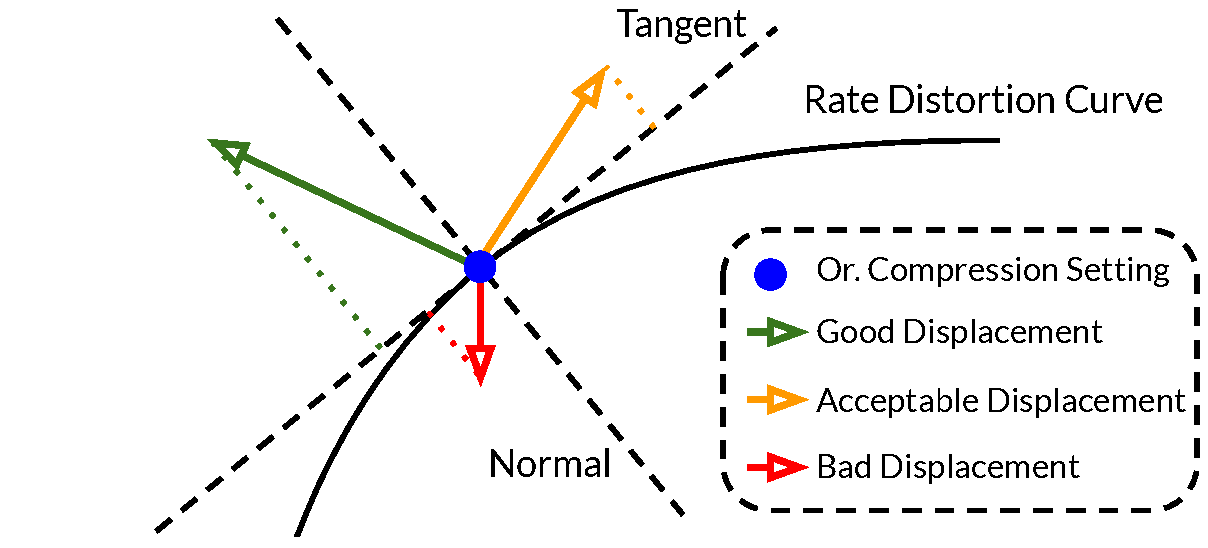
\includegraphics[width=0.9\linewidth]{revised-fig/4-critieria-of-select-tangent.pdf}
    \caption{Illustration of the geometric evaluation criterion. The rate distortion curve is evaluated between PSNR and bit rate.}
    \label{fig:projection}
\end{figure}

To address this issue, we propose a geometric evaluation criterion, as illustrated in Figure~\ref{fig:projection}. Given a target compression setting, we estimate the local tangent of the rate-distortion curve and evaluate predictors by their displacement along the normal direction. Predictors above the curve are considered better, and those with larger normal displacement are preferred, while predictors below the curve are considered worse.

The intuition behind this criterion is that the local rate-distortion curve already characterizes the ordinary tradeoff between bitrate and distortion under different error bounds. As a result, variations along the tangent direction can often be reproduced simply by adjusting the error bound and therefore do not necessarily reflect intrinsic predictor quality. In contrast, displacement along the normal direction better captures whether a predictor truly improves the rate-distortion tradeoff. This criterion is used to guide predictor selection in ASZ.

\subsection{Selecting Predictor Coefficients}\label{sec:asz:select coeff}

Selecting predictor coefficients is a core operation in ASZ.
Recall we used 4 data points to predict the target. Given a stencil pattern and an error bound, the goal is to identify the coefficient configuration that achieves the best rate–distortion tradeoff.
Algorithm~\ref{alg:asz:select coeff} shows the overall procedure, hereafter denoted as \texttt{SelectCoeff}.
% 我们根据stencil pattern收集两个统计量。分别是关于tunable variable的预测误差中的一次项系数之和和常数项之和。这两个量我们记为A和B，它们只和数据有关，和tunable variable无关，所以可以提前完成计算并复用。


% Selecting predictor coefficients is a core operation in ASZ.
% Given a stencil pattern and an error bound, the goal is to identify the coefficient configuration that achieves the best rate--distortion tradeoff.
% Algorithm~\ref{alg:asz:select coeff} shows the overall procedure.
% We first rewrite the prediction error as an affine function of the tunable coefficient.
% For each data point, this formulation produces two coefficient-independent terms, denoted as $A$ and $B$.
% These two terms depend only on the input data and the selected stencil pattern, so their joint distribution can be computed once and reused for all candidate coefficients.
% For each candidate coefficient, ASZ derives the corresponding prediction error distribution from the precomputed joint distribution of $A$ and $B$.
% It then computes the first-order entropy H$_1$ as a proxy for bitrate and derives PSNR from the estimated mean squared error.
% Finally, ASZ applies the geometric evaluation criterion in Section~\ref{sec:asz:evaluation} to compute the signed distance to the tangent.
% The candidate with the largest signed distance is selected as the final coefficient.

\begin{algorithm}[h]
\small
\caption{Select Predictor Coefficients}
\label{alg:asz:select coeff}
\KwIn{\parbox[t]{0.9\linewidth}{
Input data $D$, error bound $eb$, tangent $t$, stencil pattern $s$
}}
\KwOut{Predictor coefficients $c$}
\textcolor{blue}{\textit{// Section \ref{sec:asz:select coeff:decouple}: Precomputed Statistics.}}\\
% \tcp*[h]{Sec.\ref{sec:asz:select coeff:decouple}: Precomputed statistics}\\
$P_{A,B} \leftarrow$ EstimateJointDistribution$(D,s)$\;
$c_{\mathrm{best}} \leftarrow \emptyset$, $\Delta_{\mathrm{best}} \leftarrow -\infty$\;
\ForEach{candidate coefficient $c$}{
    \textcolor{blue}{\textit{// Section \ref{sec:asz:select coeff:decouple}: Error Distribution.}}\\
    % \tcp*[h]{Sec.\ref{sec:asz:select coeff:decouple}: Error distribution}\\
    $P_{err},mse \leftarrow$ PropagateErrorDistribution$(P_{A,B},c,eb)$\;
    \textcolor{blue}{\textit{// Section \ref{sec:asz:select coeff:H1}: Entropy-distortion-based Evaluation.}}\\
    % \tcp*[h]{Sec.\ref{sec:asz:select coeff:H1}}\\
    $h_1 \leftarrow$ ComputeEntropy$(P_{err})$\;
    $psnr \leftarrow$ ComputePSNR$(mse)$\;
    $\Delta \leftarrow$ SignedDistanceToTangent$(h_1,psnr,t)$\;
    \If{$\Delta > \Delta_{\mathrm{best}}$}{
        $\Delta_{\mathrm{best}} \leftarrow \Delta$, $c_{\mathrm{best}} \leftarrow c$\;
    }
}
\Return{$c_{\mathrm{best}}$}\;
\end{algorithm}

We first estimate a joint distribution of the input data based on the given stencil pattern, which captures the statistical relationships between neighboring data points.
This distribution is computed once and reused for all candidate coefficients.
For each candidate coefficient, we then propagate this distribution to estimate the resulting prediction error distribution and its mean squared error.
Based on the estimated error distribution, we compute the first-order entropy as a proxy for bitrate, and derive PSNR from the mean squared error.
Using the geometric evaluation criterion introduced in Section~\ref{sec:asz:evaluation}, we compute the signed distance of each candidate to the tangent, which measures its relative performance.
The coefficient with the largest distance is selected as the optimal one.

\subsubsection{Entropy-based Evaluation via H$_1$–PSNR}\label{sec:asz:select coeff:H1}\noindent

% We use H$_1$–PSNR as an efficient proxy for BR–PSNR to enable fast and reliable coefficient evaluation. In prior work, it has been widely used as a proxy for estimating bitrate, as it provides a lower bound on the achievable coding rate under some idealized assumptions, such as independent and identically distributed symbols. 

% However, in practice, we observe that H$_1$ can be larger than the actual bitrate. This discrepancy arises because the Zstandard compression in the SZ framework exploits coding dependencies between symbols, effectively reducing the coding cost below the naive entropy estimate based solely on the marginal distribution.

% Despite the fact that H$_1$ is not an accurate estimator of the true bitrate, we observe that H$_1$–PSNR curves are highly effective for distinguishing candidate coefficients. In particular, for the same stencil pattern and error bound but different coefficients, the relative ordering of H$_1$–PSNR curves closely matches that of the corresponding BR–PSNR curves. To illustrate this, we present an example dataset and compare the two types of curves under varying coefficients. As shown in Figure~\ref{fig:br-psnr-h1-psnr}, at the same error bound, the relative positions of the points induced by BR–PSNR and H$_1$–PSNR exhibit strong similarity, indicating that H$_1$–PSNR serves as a reliable proxy for coefficient selection.

% We use H$_1$–PSNR as a proxy for BR–PSNR to enable efficient coefficient evaluation.
% Here, BR–PSNR refers to the standard rate–distortion metric using actual bitrate and PSNR, while H$_1$–PSNR replaces bitrate with the first-order entropy H$_1$ of quantized prediction errors.
% Although H$_1$ is only an approximation of the true bitrate, it has been widely used due to its simplicity.
% In practice, the actual bitrate can deviate from H$_1$, as the lossless encoder exploits dependencies between symbols.
% While H$_1$ is computed based on the marginal distribution of quantized prediction errors, practical encoders such as Zstandard leverage context modeling and entropy coding to capture correlations across symbols.
% As a result, the effective coding cost can be lower than that predicted by H$_1$.

We use H$_1$–PSNR as a proxy for BR–PSNR to enable efficient coefficient evaluation. Here, BR–PSNR refers to the standard rate–distortion metric using actual bitrate and PSNR, while H$_1$–PSNR replaces bitrate with the first-order entropy H$_1$ of quantized prediction errors. Compared with directly measuring bitrate through full lossless encoding, H$_1$ can be computed much more efficiently from the prediction error distribution.

However, H$_1$ is only an approximation of the true bitrate. In practice, the actual bitrate can deviate from H$_1$ because modern lossless encoders exploit dependencies between symbols. While H$_1$ is computed solely from the marginal distribution of quantized prediction errors, practical encoders such as Zstandard further leverage context modeling and entropy coding to capture inter-symbol correlations. As a result, the effective coding cost can be lower than that predicted by H$_1$.



\begin{figure}[htb]
    \centering
    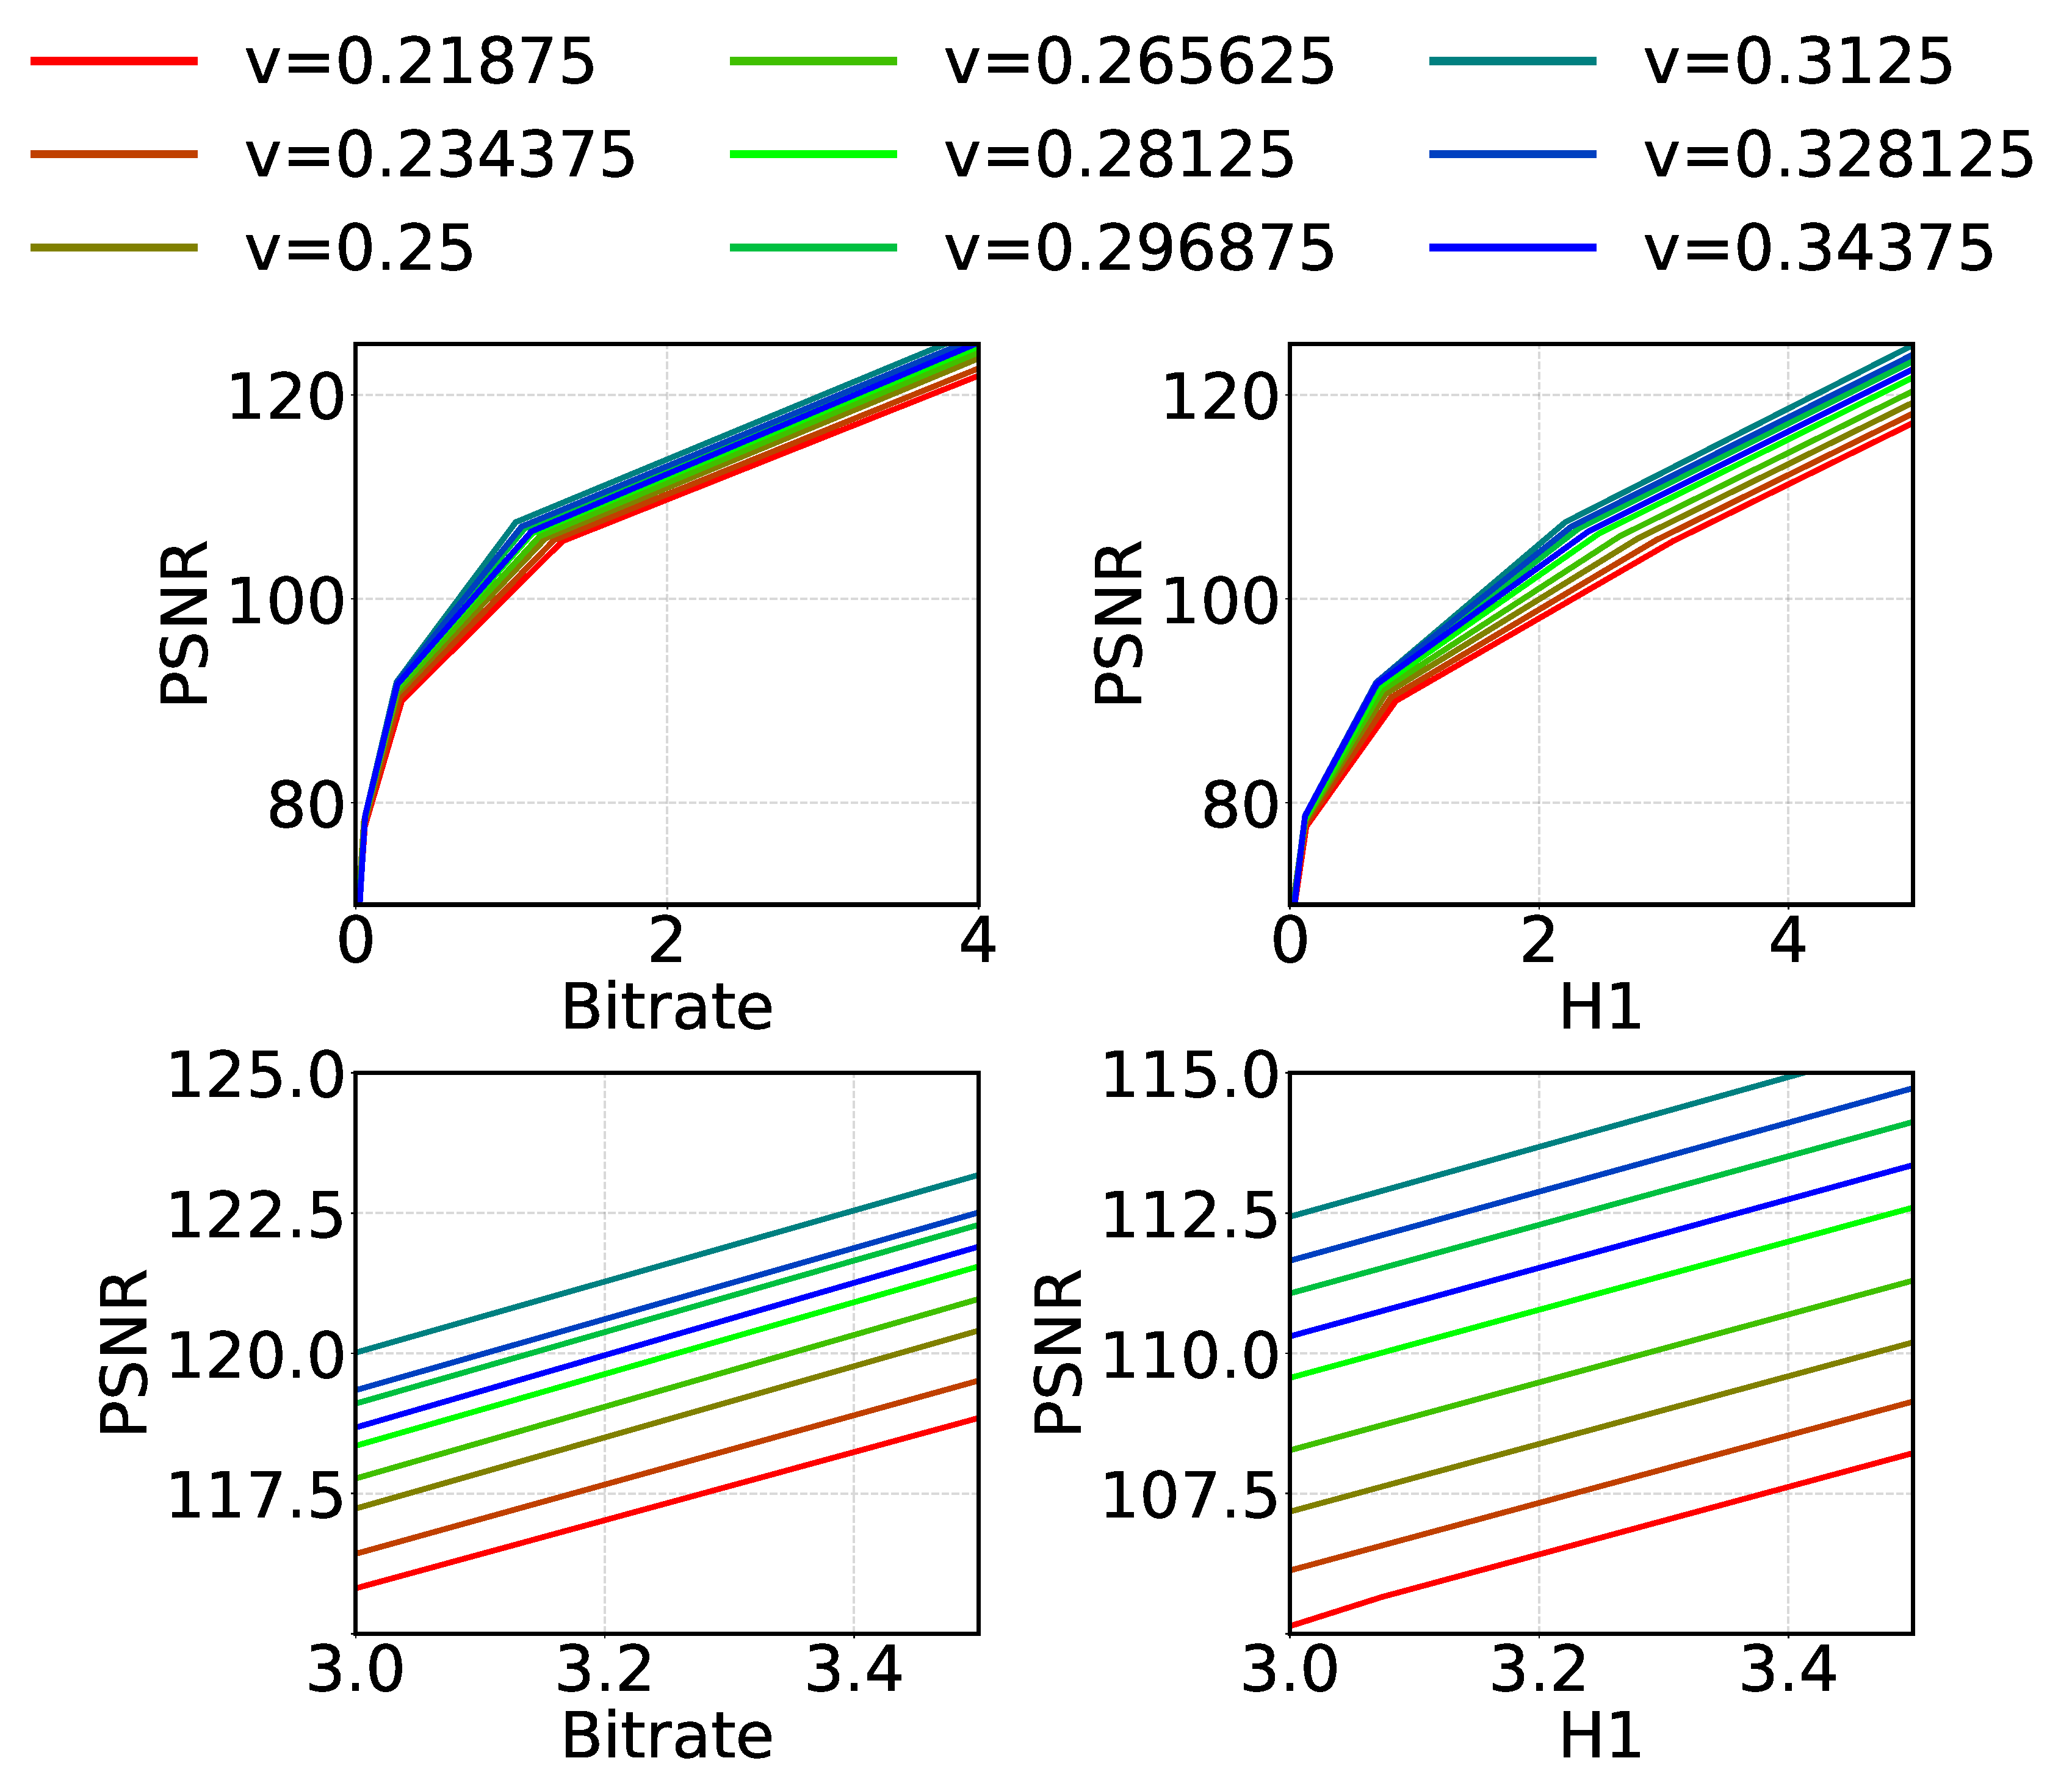
\includegraphics[width=0.8\linewidth]{figs/4/BR-PSNR和H1-PSNR.pdf}
    \caption{Comparison between BR–PSNR and H$_1$–PSNR curves. $v$ denotes the tunable variables in prediction. The second row shows zoomed-in views of the corresponding plots in the first row. These results are generated using a weather simulation dataset~\cite{kossin2004mesovortices} with the same stencil pattern. }
    \label{fig:br-psnr-h1-psnr}
\end{figure}

% It is worth noting that, while clear cross-error-bound similarity in the relative ordering of predictors can be observed in this example, such behavior is not required by our approach. In practice, comparisons are always performed at a fixed error bound.

% The discriminative power of H$_1$–PSNR curves is primarily reflected in their visual similarity to BR–PSNR curves. Therefore, we can directly apply the geometric evaluation criterion introduced in Section~\ref{sec:asz:evaluation} to select the best coefficients after estimating H$_1$ and PSNR.

Despite this discrepancy, we observe that H$_1$–PSNR is highly effective for comparing candidate coefficients.
Figure~\ref{fig:br-psnr-h1-psnr} shows that, under the same stencil pattern and error bound, the curves corresponding to different coefficients almost overlap between BR–PSNR and H$_1$–PSNR.
This indicates that H$_1$–PSNR preserves the relative ordering of candidate coefficients.
Based on this observation, we use H$_1$–PSNR as a reliable and efficient proxy for coefficient selection, and directly apply the geometric evaluation criterion from Section~\ref{sec:asz:evaluation}.


\subsubsection{Error Estimation via Precomputed Statistics}\label{sec:asz:select coeff:decouple}\noindent

% Notably, computing H$_1$ only requires the distribution of quantized prediction errors and does not depend on their ordering. This observation allows us to decouple coefficient evaluation from explicit prediction.

% To this end, we reformulate the formula of prediction error as an affine function of the tunable variables. Take Figure~\ref{fig:general sp coeff}(a) as an example, Equation~\eqref{eq:prediction formula} shows the prediction error of a variable-coefficient 1D four-point predictor, while Equation~\eqref{eq:affine form} presents its affine form.

% Both the linear coefficient $A$ and the constant term $B$ in the affine formulation are independent of the tunable variable $v$. Therefore, we can precompute their joint distribution in advance. As long as the stencil pattern remains unchanged, this joint distribution can be reused to efficiently construct the prediction error distribution for different coefficients without accessing the original data.

% Moreover, the forms of $A$ and $B$ imply that their joint distribution is typically concentrated around zero, especially when the data is locally smooth. Figure~\ref{fig:ABdata} shows example distributions of $A$, $B$, and the original data. This property further reduces the computational cost when deriving the prediction error distribution from the precomputed statistics.

Computing H$_1$ only requires the distribution of quantized prediction errors and does not depend on their ordering.
This observation allows us to decouple coefficient evaluation from explicit prediction.
Specifically, the prediction error can be reformulated as an affine function of the tunable coefficient.
For example, for the 1D four-point predictor in Figure~\ref{fig:general sp coeff}, the prediction error can be written as
$A \cdot v + B$,
where both $A$ and $B$ depend only on the input data and the stencil pattern, and are independent of $v$.
This formulation enables us to precompute the joint distribution of $A$ and $B$ once.
Then, for any candidate coefficient $v$, the corresponding prediction error distribution can be efficiently and accurately derived without accessing the original data.


\begin{figure}[htb]
    \centering
    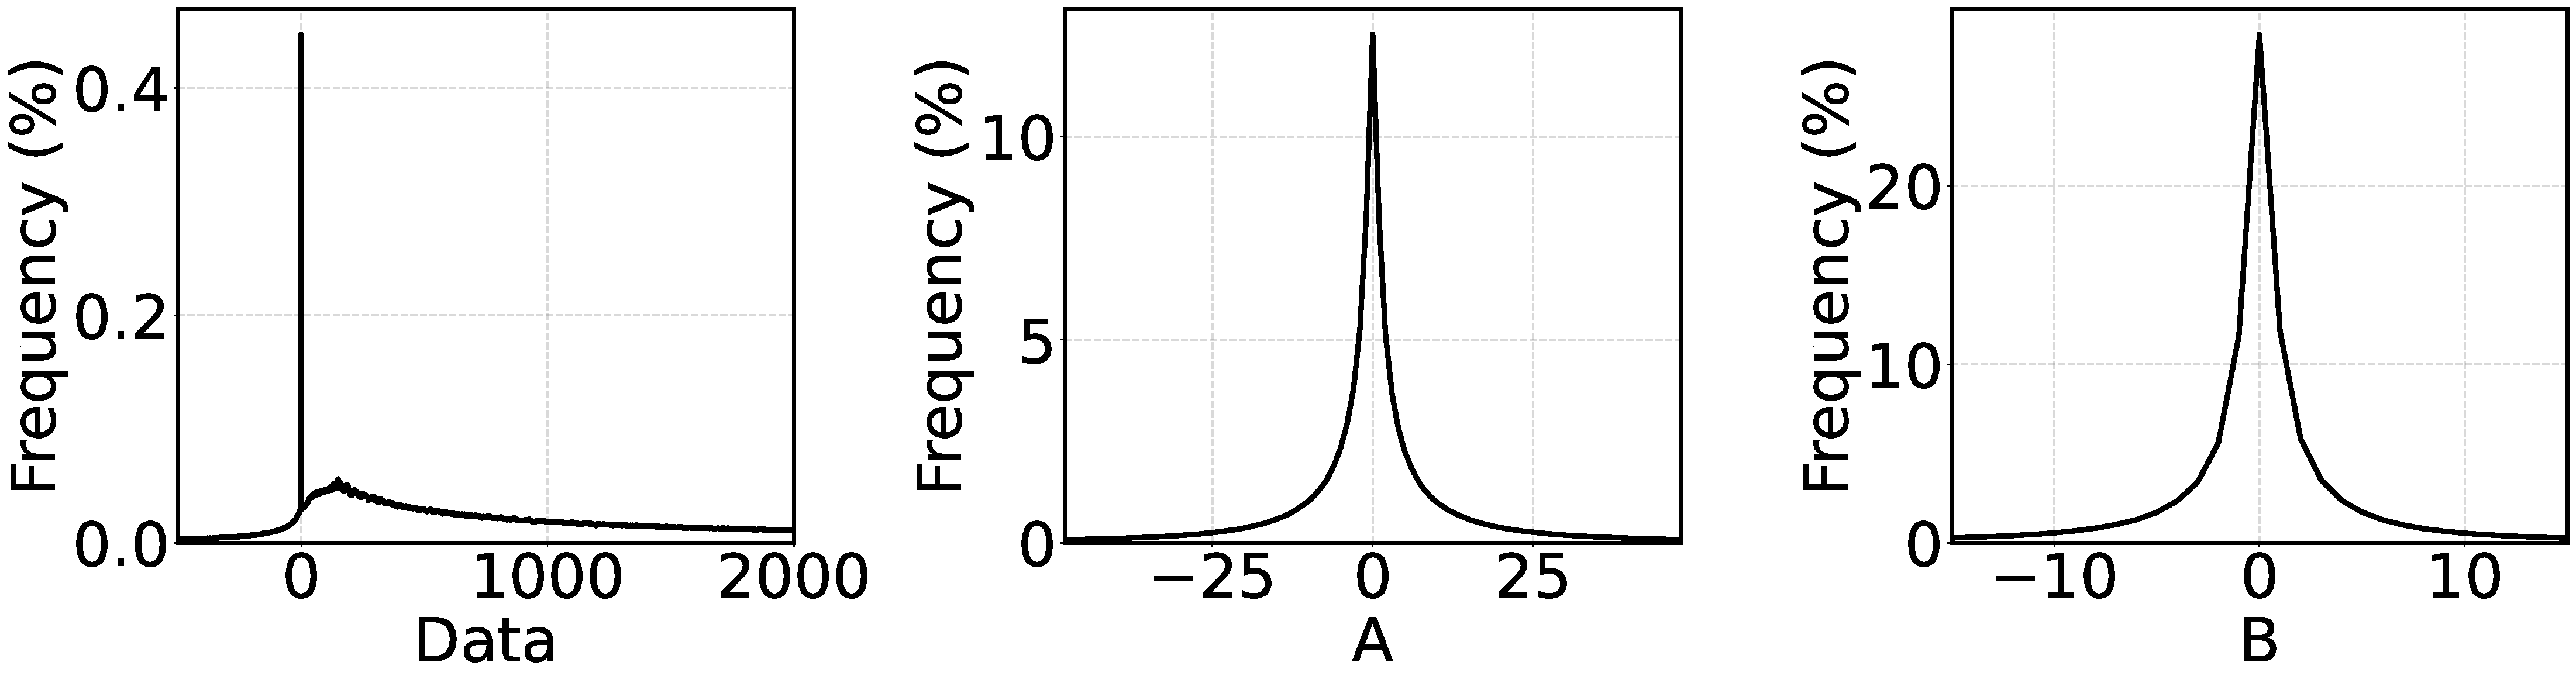
\includegraphics[width=1\linewidth]{figs/4/A、B、data的分布.pdf}
    \caption{Data distribution. Both $A$ and $B$ exhibit generalized Gaussian-like distributions, where most probability mass is concentrated near zero, allowing prediction-error distributions to be propagated with lower computational cost.}
    \label{fig:ABdata}
\end{figure}

Moreover, as shown in Figure~\ref{fig:ABdata}, the distributions of $A$ and $B$ are typically highly concentrated around zero. This implies that most probability mass naturally lies within a small range, while values with large magnitude occur infrequently. As a result, during prediction-error distribution propagation on sampled data, only a relatively small number of value combinations contribute non-negligible probability mass. This concentration substantially reduces both the computational cost and memory overhead of the propagation process.

\subsection{Estimating Tangent}\label{sec:asz:estimate tangent}

% Estimating the tangent of the rate–distortion curve at the target error bound is the first stage of ASZ. The estimated tangent is reused throughout the compression process as a reference for comparing different predictors. The corresponding pseudocode is shown in Algorithm~\ref{alg:asz:estimate tangent}.

% In ASZ, the tangent is estimated by simulating the final compression round under multiple configurations. Specifically, we consider all candidate stencil patterns and coefficients, and evaluate them at two auxiliary error bounds, one larger and one smaller than the user-specified error bound (e.g., $2\times$ and $0.5\times$). For each configuration, we estimate H$_1$ and PSNR on sampled data, and compute their averages across all candidate predictors. The tangent is then approximated using the averaged H$_1$–PSNR values at these two error bounds.


Estimating the tangent of the rate-distortion curve at the target error bound is the first stage of ASZ compression workflow.
This tangent serves as the reference direction in the geometric evaluation criterion introduced in Section~\ref{sec:asz:evaluation}, and is later reused for both stencil pattern selection and coefficient selection.
Algorithm~\ref{alg:asz:estimate tangent} shows the overall procedure.

\begin{algorithm}[h]
\small
\caption{Estimate Tangent}
\label{alg:asz:estimate tangent}
\KwIn{Input data $D$, error bound $eb$.}
\KwOut{Tangent $t$.}
$eb_1 \leftarrow 0.5 \times eb$, $eb_2 \leftarrow 2 \times eb$\;
\ForEach{$i \in \{1,2\}$}{
    $H[i] \leftarrow 0$, $\mathit{PSNR}[i] \leftarrow 0$\;
    \ForEach{stencil pattern $s$}{
        $P_{A,B} \leftarrow$ EstimateJointDistribution$(D,s)$\;
        \ForEach{candidate coefficient $c$}{
            $P_{err},mse \leftarrow$\\
            \Indp
            PropagateErrorDistribution$(P_{A,B},c,eb_i)$\;
            \Indm
            $H[i,s,c] \leftarrow$ ComputeEntropy$(P_{err})$\;
            $\mathit{PSNR}[i,s,c] \leftarrow $ ComputePSNR$(mse)$\;
        }
    }
}
$t \leftarrow \left(\overline{H[2]}-\overline{H[1]},\overline{\mathit{PSNR}[2]}-\overline{\mathit{PSNR}[1]}\right)$\;
\Return{$t$}\;
\end{algorithm}

The key idea is to approximate the local direction of the H$_1$-PSNR curve around the user-specified error bound.
To this end, ASZ evaluates candidate predictors at two auxiliary error bounds, one smaller and one larger than the target error bound, e.g., $0.5\times eb$ and $2\times eb$.
For each auxiliary error bound, ASZ considers all candidate stencil patterns and coefficient configurations.
For each configuration, H$_1$ and PSNR are estimated using the same prediction-error distribution propagation procedure described in Algorithm~\ref{alg:asz:select coeff}.
ASZ then averages the H$_1$ and PSNR values across all candidate predictors at each auxiliary error bound.
Finally, the tangent is estimated as the vector between the two averaged H$_1$-PSNR points.

% This design is motivated by robustness considerations. For example, at large error bounds, certain predictors may produce degenerate cases where H$_1$ is zero at both error bounds, typically because all quantized prediction errors vanish on the sampled data. In such cases, the estimated tangent of this predictor becomes ill-defined. By averaging over a large set of predictors, ASZ reduces the chance of such degenerate configurations and yields a more stable estimation of the tangent.

This averaging-based design improves robustness.
Estimating the tangent from a single predictor can be unstable, especially at large error bounds.
For example, a predictor may produce zero entropy at both auxiliary error bounds if all quantized prediction errors vanish on the sampled data, making its local direction ill-defined.
By aggregating the behavior of many candidate predictors, ASZ avoids relying on such degenerate cases and obtains a more stable estimate of the local rate--distortion direction.

\subsection{Selecting Stencil Patterns}\label{sec:asz:select sp}

% The second stage of ASZ is to select the stencil pattern for each round of prediction.

% From the perspective of multi-round prediction, a key challenge arises from the fact that reconstruction errors introduced in earlier rounds propagate to later rounds. These errors cannot be treated as independent noise, as they remain correlated with the underlying data due to the limited representational capacity of stencil patterns, which typically capture correlations only along specific directions. For example, a predictor designed along one direction always fails to capture correlations in other directions, leading to reconstruction errors that exhibit structured, data-dependent patterns. As a result, these errors cannot be faithfully characterized under a single-round assumption.

% Ideally, one would jointly optimize stencil patterns across all rounds to account for such interactions. However, this leads to a combinatorial explosion in the search space and requires repeated access to large volumes of data for evaluation, making it impractical in actual workflow.

% Therefore, ASZ adopts a practical strategy that evaluates stencil patterns on a per-round basis. Rather than relying purely on theoretical modeling, our approach is guided by empirical observations and carefully designed evaluation criteria to ensure that decisions made at each round remain effective in the overall multi-round compression process.


The second stage of ASZ selects the stencil pattern for each prediction round.
The goal is to identify a sequence of stencil patterns that collectively achieve good rate-distortion performance.
A key challenge arises from the multi-round nature.
Reconstruction errors introduced in earlier rounds propagate to later rounds and remain correlated with the underlying data.
This is because each stencil pattern captures correlations only along specific directions.
As a result, the effectiveness of a stencil pattern depends not only on its local behavior, but also on its interaction with patterns used in other rounds.

Ideally, stencil patterns should be jointly optimized across all rounds.
However, such joint optimization leads to a combinatorial explosion in the search space and requires repeated access to large volumes of data, which is quite impractical.
To address this, ASZ adopts a strategy that selects stencil patterns on a per-round basis while accounting for their impact on the overall process.
Algorithm~\ref{alg:asz:select sp} shows the procedure.


\begin{algorithm}[h]
\small
\caption{Select Stencil Patterns}
\label{alg:asz:select sp}
\KwIn{Input data $D$, error bound $eb$, tangent $t$}
\KwOut{Stencil pattern list $S$}
$stride \leftarrow \{1,1,1\}$, $S \leftarrow [\ ]$\;
\ForEach{round $r$ in reverse order}{
    $\Delta_{\mathrm{best}} \leftarrow -\infty$, $s_{\mathrm{best}} \leftarrow \emptyset$\;
    $eb',t' \leftarrow$ RoundSpecificAdjustment$(eb,t,r)$\;
    \ForEach{stencil pattern $s$}{
        $c \leftarrow$ SelectCoeff$(D,eb',t',s)$\;
        $br,mse \leftarrow$\\
        \Indp
        SingleRoundCompress$(D,eb',t',s,c,stride)$\;
        \Indm
        $psnr \leftarrow$ComputePSNR$(mse)$\;
        $\Delta \leftarrow$ DistanceToTangent$(br,psnr,t')$\;
        \If{$\Delta>\Delta_{\mathrm{best}}$}{
            $\Delta_{\mathrm{best}} \leftarrow \Delta$\, $s_{\mathrm{best}} \leftarrow s$\;
        }
    }
    Prepend$(S,s_{\mathrm{best}})$\;
    $stride \leftarrow$ UpdateStride$(s_{\mathrm{best}},stride)$\;
}
\Return{$S$}\;
\end{algorithm}

Specifically, ASZ processes prediction rounds in reverse order, starting from the last round and proceeding to the first.
This design prioritizes decisions that affect larger portions of data and allows later rounds to be optimized without being constrained by choices of earlier rounds.

For each round $r$, ASZ first performs a round-specific adjustment of the error bound and tangent. Specifically, ASZ reduces the error bound and flattens the tangent for upper rounds, which limits reconstruction errors introduced early in the prediction process. This helps provide more accurate reference values for lower rounds and thereby improves their prediction accuracy.

Next, ASZ iterates over all candidate stencil patterns.
For each stencil pattern $s$, it invokes Algorithm~\ref{alg:asz:select coeff} to determine the optimal coefficient configuration under the adjusted settings.
Given the stencil pattern and its selected coefficients, ASZ evaluates its performance using single-round compression on sampled data.
This step produces the estimated bitrate and mean squared error, from which PSNR is computed.
The resulting rate–distortion point is then compared, and the most suitable stencil pattern is selected as the best candidate for the current round.

After selecting the stencil pattern, ASZ prepends it to the output list $S$, ensuring that the final list follows the forward prediction order.
The stride is then updated according to the selected stencil pattern, which affects how subsequent rounds access data.

% ASZ adopts the following strategies for precise stencil pattern selection.

% \begin{itemize}
% \item Stencil patterns are selected in reverse order of prediction. This is motivated by the observation that the amount of newly compressed data generated at each round roughly doubles compared with the previous round. As a result, the choices of stencil patterns in later rounds have more significant impact on overall compression performance. In the reverse selection process, stencil patterns in later rounds are not constrained by earlier rounds, allowing more optimal choices. Although earlier rounds have reduced flexibility, their contribution to the overall compression performance is negligible.

% \item Stencil patterns are evaluated using single-round compression on sampled data rather than relying on H$_1$-PSNR criterion. This is because H$_1$-based evaluation does not always preserve the relative ranking of stencil patterns observed in actual BR-PSNR results. We also investigated higher-order entropy metrics, such as H$_2$-PSNR curves, where H$_2$ means the discrete second-order conditional entropy. This may reflect potential multi-symbol coding effects in Zstandard, but found them to be less reliable in practice.

% \item Since quantized prediction errors may still exhibit spatial correlation, we consider not only different stencil patterns but also different storage orders of the quantized errors. This allows the compression backend to better exploit potential dependencies among symbols.

% \item We bias the selection toward producing more concentrated reconstruction errors in earlier rounds to mitigate the propagation of structured errors in subsequent rounds with larger data volumes. Similar ideas have been adopted in SZ3 and QoZ, where smaller error bounds are used for earlier rounds. Building on this, ASZ further adjusts the distribution of reconstruction errors in earlier rounds by applying flatter tangents when comparing candidate predictors.
% \end{itemize}

% The corresponding pseudocode is shown in Algorithm~\ref{alg:asz:select sp}.

\subsection{Block-wise Compression in ASZ}\label{sec:asz:compress}

Finally, ASZ performs compression in a block-wise manner. The data is partitioned into blocks, where the block shape is determined based on the selected sequence of stencil patterns in Section~\ref{sec:asz:select sp}. The pseudocode is shown in Algorithm~\ref{alg:asz:compress}.

\begin{algorithm}[h]
\small
\caption{Compress}
\label{alg:asz:compress}
\KwIn{\parbox[t]{0.9\linewidth}{
Input data $D$, error bound $eb$,\\
tangent $t$, stencil patterns $S$
}}
\KwOut{Compressed bitstream $B$}
$Blocks \leftarrow$ PartitionIntoBlocks$(D)$, $C \leftarrow [\ ]$ \;
\ForEach{round $r$}{
    $\mathit{QB}[r] \leftarrow [\ ]$\;
}
\ForEach{$Block \in Blocks$}{
    \ForEach{round $r$}{
        $s \leftarrow S[r]$\;
        $stride \leftarrow$ GetStride$(S,r)$\;
        $eb',t' \leftarrow$ RoundSpecificAdjustment$(eb,t,r)$\;
        $c \leftarrow$ SelectCoeff$(Block,eb',t',s,stride)$\;
        Append$(C,c)$\;
        $qb \leftarrow$ PredictAndQuantize$(Block,eb',s,c,stride)$\;
        Append$(\mathit{QB}[r],qb)$\;
    }
}
\ForEach{round $r$}{
    $Huff[r] \leftarrow$ HuffmanEncode$(\mathit{QB}[r])$\;
}
$C \leftarrow$ HuffmanEncode$(C)$\;
$B \leftarrow$ ZstdCompress$(Huff,S,C)$\;
\Return{$B$}\;
\end{algorithm}

First, the input data is partitioned into blocks. This block-wise design improves data locality and allows predictor coefficients to adapt to local data characteristics.

For each block and each prediction round, ASZ retrieves the selected stencil pattern and adjusts the error bound and tangent using the same strategy described in Algorithm~\ref{alg:asz:select sp}. Given these round-specific settings, ASZ selects predictor coefficients based on the local statistics of the current block. At this stage, part of the block has already been compressed and reconstructed, which may change the optimal predictor coefficients compared with those estimated during the previous exploration stage. Since coefficient selection in ASZ is computationally inexpensive, the coefficients can be efficiently re-estimated during block-wise compression to better adapt to reconstructed local data.

ASZ then performs prediction and quantization using the selected stencil pattern and coefficients, producing quantized prediction errors. After all blocks are processed, ASZ encodes the quantized prediction errors in a round-wise manner, instead of encoding all errors together as in the traditional SZ compression framework. Specifically, errors from the same prediction round are encoded together using Huffman coding, because their distributions tend to be more consistent across different blocks within the same round due to the shared layer-specific error bound and tangent adjustment strategy, while the distributions across different rounds may vary significantly.

Finally, the encoded prediction errors, selected stencil patterns, and predictor coefficients are further compressed using Zstandard to generate the final byte stream~\cite{liang2022sz3}.

% Within each block, the previously selected stencil pattern sequence is reused, while the predictor coefficients are re-estimated locally. This is because, at this stage, the reconstructed lossy data is available, and the optimal coefficients may differ slightly from those estimated earlier.

% Finally, during entropy coding, quantized prediction errors from the same round but different blocks are encoded independently. This is motivated by the observation that their distributions may vary across rounds, but tend to be similar across different blocks within each round. This localized encoding strategy slightly improves compression efficiency by better matching the underlying distributions.

% First, the input data is partitioned into blocks. 
% This block-wise design improves data locality and allows predictor coefficients to adapt to local data characteristics. 
% ASZ then initializes a list for storing selected predictor coefficients and a set of buffers for collecting quantized prediction errors from different prediction rounds.

% Compression proceeds over all blocks and prediction rounds. 
% For each block and each prediction round, ASZ retrieves the selected stencil pattern, and adjusts the error bound and tangent using the same strategy described in Algorithm~\ref{alg:asz:select sp}. 
% Given these settings, ASZ selects predictor coefficients based on the local statistics of the current block. At this stage, part of the block has already been compressed and reconstructed, which may change the optimal predictor coefficients compared with those estimated during the previous exploration stage. Since coefficient selection in ASZ is computationally inexpensive, the coefficients can be efficiently re-estimated during block-wise compression to better adapt to the reconstructed local data.
% The selected coefficients are recorded as metadata for later decoding. 
% ASZ then performs prediction and quantization using the selected stencil pattern and coefficients, producing quantized prediction errors. 

% Instead of encoding these errors together, ASZ accumulates quantized errors from the same prediction round across all blocks.
% After all blocks are processed, ASZ encodes the quantized prediction errors in a round-wise manner. 而不是像SZ compression framework那样全部encode 在一起。
% Specifically, errors from the same round are encoded together using Huffman coding, because their distributions tend to be more consistent across blocks within the same round, while differing more significantly across rounds. 
% Finally, the encoded prediction errors, selected stencil patterns, and predictor coefficients are compressed using Zstandard to generate the final byte stream~\cite{liang2022sz3}.

% Two design choices are particularly important in this stage. 
% First, although stencil patterns are fixed after the stencil-pattern selection stage, predictor coefficients are selected separately for each block. 
% This allows ASZ to adapt to local data variations without repeating the more expensive global stencil-pattern search. 
% Second, quantized prediction errors are encoded per round rather than per block. 
% This improves lossless compression efficiency by grouping symbols with more similar distributions.

% First, the input data is partitioned into a set of blocks.
% This design improves locality and allows coefficient selection to adapt to local data characteristics.
% ASZ then initializes a list to store predictor coefficients and a set of buffers to collect quantized prediction errors for each round.
% The compression proceeds by iterating over all blocks and all prediction rounds.
% For each block and each round, ASZ retrieves the corresponding stencil pattern and its stride, and performs a round-specific adjustment of the error bound and tangent.
% Given these settings, ASZ invokes \texttt{SelectCoeff} to re-estimate the optimal predictor coefficients based on the local block data.
% The selected coefficients are recorded for later encoding.
% Using the selected stencil pattern and coefficients, ASZ performs prediction and quantization to generate quantized prediction errors.
% These errors are accumulated separately for each round across all blocks.
% After processing all blocks, ASZ performs entropy coding in a round-wise manner.
% Specifically, quantized prediction errors from the same round are encoded together using Huffman coding.
% This design leverages the observation that error distributions tend to be more consistent across different blocks within the same round, while varying significantly across rounds.
% Finally, the encoded prediction errors, stencil patterns, and predictor coefficients are further compressed using Zstandard to produce the final byte stream~\cite{liang2022sz3}.

% Two design choices are particularly important in this stage.
% First, although the stencil patterns are fixed after the previous stage, predictor coefficients are re-estimated for each block.
% This is because local data characteristics may differ, and more accurate coefficients can be obtained when reconstructed data is available.
% Second, entropy coding is performed per round rather than per block, which improves compression efficiency by better matching symbol distributions.